\documentclass[5pt]{extarticle}
\usepackage[top=0in, bottom=0.1in, left=0.1in, right=0.1in]{geometry} % Minimal margins
\usepackage{amsmath,amssymb,amsthm}
\usepackage{enumitem}
\usepackage{graphicx}
\usepackage{ragged2e}
\usepackage[absolute,overlay]{textpos}
\usepackage{array}
\usepackage{booktabs}
\usepackage{multicol}
\usepackage{setspace}
\usepackage{fancyvrb}
\usepackage{titlesec}
\usepackage{xcolor}
\usepackage{microtype}

% Configure microtype for more condensed text
\microtypesetup{tracking=true, letterspace=-40}
\DisableLigatures{encoding = *, family = * }

% Compress inter-word spacing
\fontdimen2\font=2pt  % inter-word space
\fontdimen3\font=-1pt  % inter-word stretch
\fontdimen4\font=1pt  % inter-word shrink
\fontdimen7\font=1pt  % extra space

% Define a custom smaller font size
\makeatletter
\newcommand{\tinyfont}{\@setfontsize\tinyfont{4pt}{2pt}}
\makeatother

% Replace \scriptsize with \tinyfont in document where needed
\let\oldscriptsize\scriptsize
\renewcommand{\scriptsize}{\tinyfont}

% Fix horizontal spacing
\setstretch{0.85}
\pagestyle{empty}
\setlength{\parindent}{0pt}
\setlength{\parskip}{0.5pt plus 0.1pt minus 0.1pt}

% Additional horizontal compression
\setlength{\tabcolsep}{1pt}  % Reduce table column separation
\renewcommand{\arraystretch}{0.8} % Compress table rows vertically

% Reduce spacing in lists
\setlist{noitemsep,topsep=0pt,parsep=0pt,partopsep=0pt,leftmargin=*}
\AtBeginEnvironment{enumerate}{\setlength{\itemsep}{-2pt}}
\AtBeginEnvironment{itemize}{\setlength{\itemsep}{-2pt}}

% Reduce spacing in multicols
\setlength{\multicolsep}{0pt}
\setlength{\columnsep}{3pt}

% Compact section titles
\titlespacing*{\section}{0pt}{0pt}{0pt}
\titlespacing*{\subsection}{0pt}{0pt}{0pt}

% Custom commands for algorithm blocks
\newcommand{\algoblock}[3]{%
  \begin{minipage}[t]{#1\textwidth}
    \setlength{\baselineskip}{0.8\baselineskip}
    \vspace{0pt}\textbf{#2}\\[0.3ex]
    #3
  \end{minipage}
}

\newcommand{\imageblock}[2]{%
  \begin{minipage}[t]{#1\textwidth}
    \vspace{0pt}\includegraphics[width=\linewidth]{#2}
  \end{minipage}
}

\newcommand{\theoremblock}[3]{%
  \begin{minipage}[t]{#1\textwidth}
    \setlength{\baselineskip}{0.8\baselineskip}
    \vspace{0pt}\textbf{#2}\\[0.3ex]
    \justifying
    #3
  \end{minipage}
}

\begin{document}

%%%%%%%%%%%%%%%%%%%%%%%%%%%%%%%%%%%%%%%%%%%%%%
% Title page
\begin{titlepage}
    \centering
    \vspace*{30px}
    {\Huge \textbf{Algorithms - CheatSheet}}\\[15px] 
    {\LARGE IN~BA4 - Ola Nils Anders Svensson}\\[15px]
    {\Large Notes by Ali EL AZDI}\\[10px]
    \vfill
    \begin{minipage}{0.8\textwidth}
        \normalsize
        \begin{justify}
            \textit{This is a cheat sheet for the Algorithms midterm exam. For suggestions, contact me on Telegram (\texttt{elazdi\_al}) or via EPFL email (\texttt{ali.elazdi@epfl.ch}).}
        \end{justify}
    \end{minipage}\\
    \vspace{40px}
    {\large March 25th, 2025}
    \vspace{40px}
\end{titlepage} 

%%%%%%%%%%%%%%%%%%%%%%%%%%%%%%%%%%%%%%%%%%%%%%
\tiny
\vspace*{-13px}
% First row - Asymptotic Notation and Master Theorem
\theoremblock{0.3}{\scriptsize Asymptotic Notation}{
    \scriptsize
\textbf{Big-O}\\[1px]
If $\exists c>0$ and $\exists n_0>0$, $0\le f(n)\le c\cdot g(n)$ $\forall n\ge n_0$, then $f(n)=O(g(n))$.\\[1px]
\textbf{Big-Omega}\\[1px]
If $\exists c>0$ and $\exists n_0>0$, $0\le c\cdot g(n)\le f(n)$ $\forall n\ge n_0$, then $f(n)=\Omega(g(n))$.\\[1px]
\textbf{Big-Theta}\\[1px]
If $f(n)=O(g(n))$ and $f(n)=\Omega(g(n))$, then $f(n)=\Theta(g(n))$.
} 
\hfill
\theoremblock{0.6}{\scriptsize Master Theorem}{
    \scriptsize
If $T(n) = a\, T\left(\frac{n}{b}\right) + f(n)$, where $a \geq 1$, $b > 1$, and $f(n)$ is asymptotically positive. The solution depends on comparing $f(n)$ to $n^{\log_b a}$:
\begin{enumerate}[noitemsep]
    \item \textbf{Case 1:} If $f(n) = O(n^{\log_b a - \epsilon})$ for some $\epsilon > 0$, then $T(n) = \Theta(n^{\log_b a})$.
    \item \textbf{Case 2:} If $f(n) = \Theta(n^{\log_b a})$, then $T(n) = \Theta(n^{\log_b a}\log n)$.
    \item \textbf{Case 3:} If $f(n) = \Omega(n^{\log_b a + \epsilon})$ for some $\epsilon > 0$, and if $a\, f\left(\frac{n}{b}\right) \leq c\, f(n)$ for some $c < 1$ and all sufficiently large $n$, then $T(n) = \Theta(f(n))$.
\end{enumerate}
\noindent
\vspace{-20px}
\begin{center}
Common case - if $f(n) = \Theta(n^d)$ for some exponent $d$:
\end{center}
\vspace{-8px}
\begin{enumerate}[noitemsep]
    \item If $\frac{a}{b^d} < 1$ (or $d > \log_b a$), then $T(n) = \Theta(n^d)$.
    \item If $\frac{a}{b^d} = 1$ (or $d = \log_b a$), then $T(n) = \Theta(n^d \log n)$.
    \item If $\frac{a}{b^d} > 1$ (or $d < \log_b a$), then $T(n) = \Theta(n^{\log_b a})$.
\end{enumerate}
} 
\fbox{%
  \algoblock{0.3}{\scriptsize Insertion Sort}{
    \scriptsize
    \begin{minipage}{0.45\textwidth}
    \begin{enumerate}[itemsep=2pt]
      \item \textbf{Select the key}\\ 
            Begin with the second element (at index 1) as the \textit{key}.
      \item \textbf{Compare and Shift}\\ 
            Compare the key with elements in the sorted section (to its left).
    \end{enumerate}
    \end{minipage}
    \begin{minipage}{0.45\textwidth}
        \imageblock{1.2}{images/insertion-sort.png}
    \end{minipage}
    \begin{enumerate}[itemsep=2pt]
      \item[3.] \textbf{Shift Elements}\\ 
            If an element is greater than the key, shift that element one position to the right.
      \item[4.] \textbf{Insert the Key}\\ 
            Once an element less than or equal to the key is found (or you reach the start), insert the key immediately after that element.
      \item[5.] \textbf{Repeat}\\ 
            Move forward to the next element, treating it as the new key, and repeat until the array is sorted.
    \end{enumerate}
    \vspace{1ex}
    \textit{Time Complexity:} Worst-case \(O(n^2)\), Best-case \(O(n)\).\\
    \textit{Space Complexity:} \(O(n)\).\\[1ex]
  }%
} 
\fbox{
\algoblock{0.65}{\scriptsize Maximum Subarray Problem}{
\scriptsize
\begin{minipage}[t]{0.75\textwidth}
\textbf{Problem:} Find contiguous subarray with largest sum
    \begin{enumerate}[noitemsep]
        \scriptsize
        \item \textbf{Divide and Conquer Approach:} \\
        \begin{minipage}[t]{0.45\textwidth}
        \scriptsize
        \textbf{Divide:} Split array at midpoint\\
        $\text{mid} = \lfloor(\text{low} + \text{high})/2\rfloor$\\[3pt]
        
        \textbf{Conquer:} Find maximum subarrays recursively\\
        1. Left max: in $A[\text{low}...\text{mid}]$\\
        2. Right max: in $A[\text{mid}+1...\text{high}]$\\
        3. Crossing max: spans the midpoint\\[3pt]
        
        \textbf{Combine:} Return the largest of the three\\
        $\max(\text{left\_max}, \text{right\_max}, \text{crossing\_max})$
        \end{minipage}
        \hspace{10px}
        \begin{minipage}[t]{0.45\textwidth}
        \vspace{-10pt}
            \imageblock{1.0}{images/max-subarray.png}
        \end{minipage}\\
        \item \textbf{Finding the Crossing Maximum:}\\
        1. Find maximum suffix in left half (from mid down to low)\\
        2. Find maximum prefix in right half (from mid+1 up to high)\\
        3. Crossing max = max suffix + max prefix
    \end{enumerate}
    \justifying
    \textit{Time Complexity:} $\Theta(n\log n)$ due to $T(n) = 2T(n/2) + \Theta(n)$\\
    \textit{Space Complexity:} $O(\log n)$ for recursion stack
\end{minipage}
\begin{minipage}[t]{0.2\textwidth}
\vspace{0pt}
\imageblock{1.2}{images/max-subarray-crossing.png}
\end{minipage}
}} \\
\fbox{
    \begin{minipage}[t]{0.25\textwidth}
        \scriptsize
        \textbf{Stack Operations}\\
        \textbf{Stack-Empty(S):} \textit{Time: O(1), Auxiliary Space: O(1)}\\[2px]
        1. Returns TRUE if the stack is empty.\\
        2. Returns FALSE otherwise.\\[2pt]
        \textbf{Push(S, x):} \textit{Time: O(1), Auxiliary Space: O(1)}\\
        1. Adds element x to the top of stack S.\\
        2. Increments the stack pointer.\\[2pt]
        \textbf{Pop(S):} \textit{Time: O(1), Auxiliary Space: O(1)}\\
        1. If Stack-Empty(S), return error "underflow".\\
        2. Otherwise, remove and return the top element.\\
        3. Decrements the stack pointer.\\[2pt]
        \textbf{Stack Implementation:}\\
        1. Elements are stored in a simple array\\
        2. S.top: Index of the topmost element\\
        3. An empty stack has S.top = 0 or S.top = -1 (implementation dependent)\\
        
        \textit{Overall Space Complexity:} \(O(n)\) for a stack of size n
    \end{minipage}
} 

\fbox{
\algoblock{0.34}{\scriptsize Strassen's Matrix Multiplication \vspace{-4px}}{
    \begin{enumerate}[noitemsep]
        \scriptsize
        \item \textbf{Divide:} Partition each of \(A, B, C\) into four \(\tfrac{n}{2} \times \tfrac{n}{2}\) submatrices: \vspace{-5px}
        \[
        \begin{pmatrix}
            C_{11} & C_{12} \\
            C_{21} & C_{22}
        \end{pmatrix}
        \;=\;
        \begin{pmatrix}
            A_{11} & A_{12} \\
            A_{21} & A_{22}
        \end{pmatrix}
        \cdot
        \begin{pmatrix}
            B_{11} & B_{12} \\
            B_{21} & B_{22}
        \end{pmatrix}.
        \]
    \begin{minipage}[t]{0.45\textwidth}
        \scriptsize
        \vspace{-8px}
        \item  \textbf{Conquer:} Compute 7 products (recursively on \(\tfrac{n}{2} \times \tfrac{n}{2}\) matrices):
        \[
        \begin{aligned}
        M_1 &:= (A_{11} + A_{22})(B_{11} + B_{22}), \\
        M_2 &:= (A_{21} + A_{22}) \, B_{11}, \\
        M_3 &:= A_{11} \,(B_{12} - B_{22}), \\
        M_4 &:= A_{22} \,(B_{21} - B_{11}), \\
        M_5 &:= (A_{11} + A_{12}) \, B_{22}, \\
        M_6 &:= (A_{21} - A_{11}) \,(B_{11} + B_{12}), \\
        M_7 &:= (A_{12} - A_{22}) \,(B_{21} + B_{22}).
        \end{aligned}
        \]
        \end{minipage}
        \hfill
        \begin{minipage}[t]{0.45\textwidth}
        \scriptsize
        \vspace{-8px}
        \item \textbf{Combine:} Assemble the resulting submatrices to form \(C\): 
        \[
        \begin{aligned}
        C_{11} &= M_1 + M_4 - M_5 + M_7, \\
        C_{21} &= M_2 + M_4, \\
        C_{12} &= M_3 + M_5, \\
        C_{22} &= M_1 + M_3 - M_2 + M_6.
        \end{aligned}
        \]
            \textit{Time Complexity:} \(O(n^{\log_2 7}) \approx O(n^{2.81})\)\\
    \textit{Space Complexity:} \(O(n^2)\)
        \end{minipage}
    \end{enumerate}
    \vspace{0.5ex}
    \justifying
}} 
\fbox{
    \begin{minipage}[t]{0.31\textwidth}
        \scriptsize
        \textbf{Queue Operations}\\        
        \textbf{Queue-Empty(Q):}\\[2px]
        1. Returns TRUE if the queue is empty (Q.head = Q.tail).\\
        2. Returns FALSE otherwise.\\[2pt]
        \textbf{Enqueue(Q, x):}\\
        1. Adds element x to the rear of queue Q.\\
        2. Q[Q.tail] = x\\
        3. Q.tail = Q.tail + 1 (or wrap around if using circular array)\\[2pt]
        \textbf{Dequeue(Q):}\\
        1. If Queue-Empty(Q), return error "underflow".\\
        2. Otherwise, remove and return the element at the front.\\
        3. x = Q[Q.head]\\
        4. Q.head = Q.head + 1 (or wrap around)\\
        5. Return x\\[2pt]
        \textbf{Queue Implementation:}\\
        1. Q.head: Index of the front element\\
        2. Q.tail: Index where next element will be inserted\\
        3. In a circular array, indices wrap around\\
        4. Leave one slot empty to distinguish full/empty states

        \textit{Time Complexity:} \(O(1)\) for all operations \quad \textit{Space Complexity:} \(O(n)\)\\
    \end{minipage}
} \\
\fbox{
\algoblock{0.55}{\scriptsize Merge Sort}{
    \scriptsize
    \begin{minipage}[t]{0.6\textwidth}
    \begin{enumerate}[noitemsep]
        \item \textbf{Divide}: Split the array evenly into two smaller subarrays, and continue dividing recursively.
        \item \textbf{Sort (Recursively)}: Apply merge sort recursively on each subarray until each has only one element (base case).
        \item[] 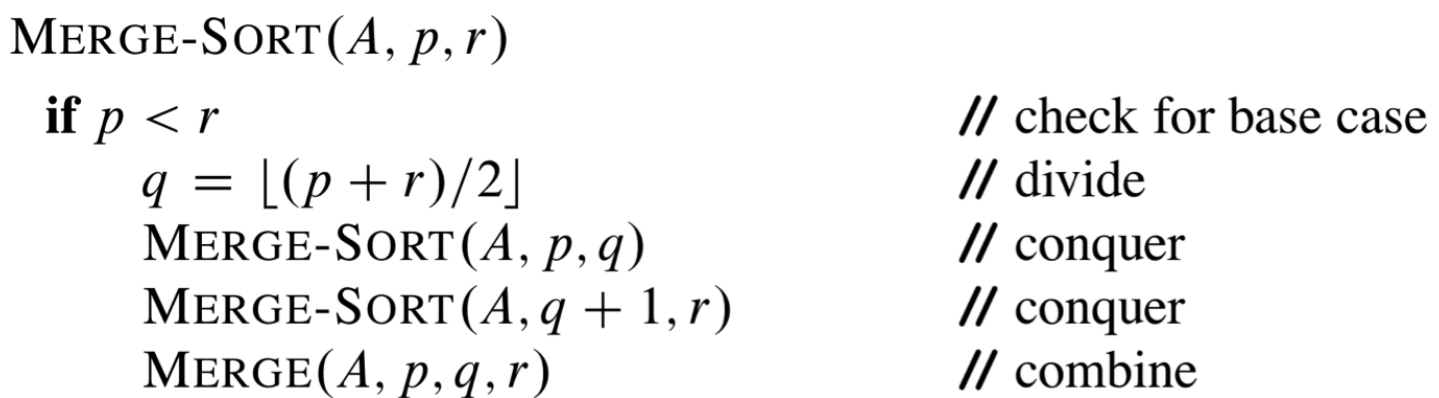
\includegraphics[width=0.75\linewidth]{images/merge-sort.png}

        \item \textbf{Merge}: Combine the two sorted subarrays into a single sorted array:
        \begin{enumerate}[noitemsep]
            \item Initializing pointers at the start of each subarray.
            \item Comparing the elements pointed to, and appending the smaller one into a new array.
            \item Advancing the pointer in the subarray from which the element was chosen.
            \item Repeating this process until all elements in both subarrays are merged into the sorted array.
        \end{enumerate}
    \end{enumerate}
    \justifying
    \textit{Merge Cost Complexity:} \(O(n)\) per merge operation.\\
    \textit{Time Complexity:} \(O(n \log n)\)\\
    \textit{Space Complexity:} \(O(n)\)
    \end{minipage}
    \hfill
    \begin{minipage}[t]{0.35\textwidth}
        \vspace{0pt}
        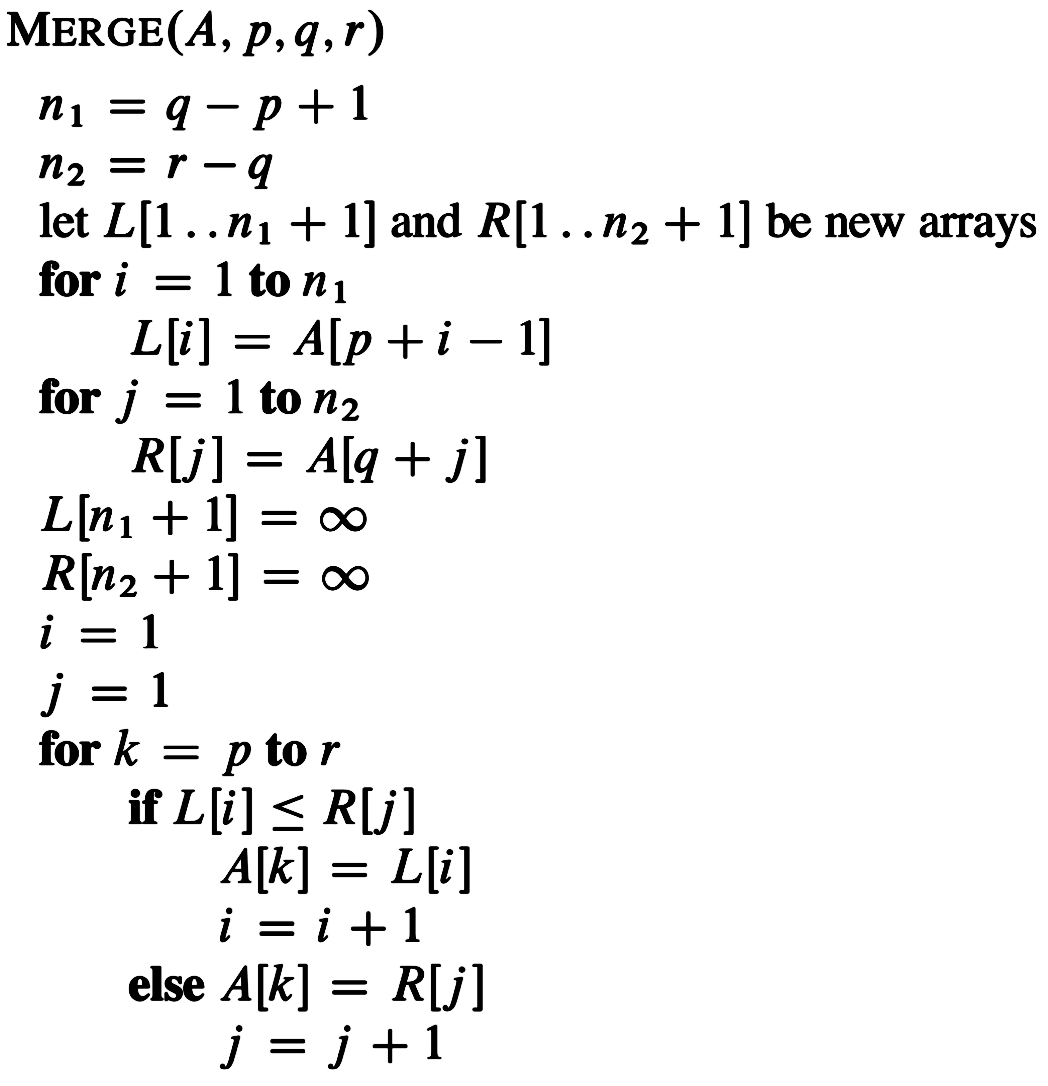
\includegraphics[width=1\linewidth]{images/merge.png}
    \end{minipage}
}
} 
\hfill
\fbox{
    \algoblock{0.4}{\scriptsize Priority Queue}{
        \scriptsize
        Maintains a dynamic set of elements with associated priority values (keys).\\
        
        \textbf{Maximum(S):} Return element of S with highest priority (return A[1], complexity $O(1)$)\\
        
        \textbf{Insert(S,x):} Insert element x into set S\\
        1. Increment the heap size\\
        2. Insert a new node in the last position in the heap, with key $-\infty$\\
        3. Increase the $-\infty$ value to key using Heap-Increase-Key\\
        
        \textbf{Extract-Max(S):} Remove and return element of S with highest priority\\
        1. Make sure heap is not empty\\
        2. Make a copy of the maximum element (the root)\\
        3. Make the last node in the tree the new root\\
        4. Re-heapify the heap, with one fewer node\\
        5. Return the copy of the maximum element\\
        
        \textbf{Increase-Key(S,x,k):} Increase the value of element x's key to the new value k\\
        1. Make sure key $\geq$ A[i]\\
        2. Update A[i]'s value to key\\
        3. Traverse the tree upward comparing new key to the parent and swapping if necessary\\
        \textit{Time Complexity:} Insert, Extract-Max, Increase-Key: $O(\log n)$ \quad Maximum: $O(1)$
        \textit{Space Complexity:} $O(n)$}} \\
\fbox{
\algoblock{0.5}{\scriptsize Heap}{
    \scriptsize
    \begin{minipage}[t]{0.65\textwidth}
        \fbox{
            \begin{minipage}[t]{1.05\textwidth}
                \scriptsize
                Root is A[1] \;
                Left(i) = 2i \; 
                Right(i) = 2i + 1 \;
                Parent(i) =$\lfloor i/2 \rfloor$
            \end{minipage}
        }
        \textbf{\scriptsize Max-Heapify (heapify subtree rooted at i)}\\
        1. Starting at the root\\
        2. Compare A[i], A[Left(i)], A[Right(i)]\\
        3. If necessary, swap A[i] with the largest of the two children\\
        4. \textbf{Max-Heapify} the swapped child\\
        5. Continue comparing and swapping down the heap until subtree rooted at i is max-heap
        \textit{Time Complexity:} \(O(\log(n))\) \quad \textit{Space Complexity:} \(O(n)\) including heap array, \(O(1)\) auxiliary
        
        \textbf{\scriptsize Max-Heap-Insert (insert new key into heap)}\\
        1. Increase heap size: A.heap-size = A.heap-size + 1\\
        2. Set the last element to negative infinity: A[A.heap-size] = $-\infty$\\
        3. Call Max-Heap-Increase-Key to update to the correct value\\
        \textit{Time Complexity:} \(O(\log n)\) \quad \textit{Space Complexity:} \(O(n)\) including heap array, \(O(1)\) auxiliary
        
        \textbf{\scriptsize Max-Heap-Increase-Key (increase key at position i)}\\
        1. Ensure new key is larger than current: if key < A[i] then error\\
        2. Set A[i] = key\\
        3. Compare with parent and swap if necessary: while i > 1 and A[Parent(i)] < A[i]\\
        4. Exchange A[i] with A[Parent(i)]\\
        5. Set i = Parent(i) and continue upward\\
        \textit{Time Complexity:} \(O(\log n)\) \quad \textit{Space Complexity:} \(O(n)\) including heap array, \(O(1)\) auxiliary
        
        \textbf{\scriptsize Build-Max-Heap (build a max-heap from an array)}
        1. Start from the last non-leaf node at index \(\frac{n}{2} - 1\)\\
        2. Move upwards to the root (index \(0\)) and:\\
        \quad a. \textbf{Max-Heapify} the current node\\
        \quad b. Ensure the subtree rooted here satisfies max-heap property\\
        3. Repeat until the root node is processed\\
        4. After completion, array \(A\) represents a valid max heap\\
        \textit{Time Complexity:} \(O(n)\) \quad \textit{Space Complexity:} \(O(n)\) including heap array, \(O(1)\) auxiliary\\
        \textbf{\scriptsize Heap Sort}\\[-1px]
        \textbf{1. Build a Max Heap:}\\
        a. Convert the given array into a max heap\\
        b. Start from the last non-leaf node and heapify upwards\\
        c. Ensure each parent node is greater than its children\\
        \textbf{2. Extract Maximum Elements:}\\
        a. Swap the root (maximum value) with the last element\\
        b. Reduce heap size by one to exclude the last element\\
        c. Heapify the root to maintain max heap property\\
        d. Repeat until heap size becomes 1\\
        \textbf{3. Final Sorted Array:}\\
        a. After extraction, the sorted array in ascending order is obtained\\
        b. Maximum elements are placed at the end\\
        \textit{Time Complexity:} \(O(n\log n)\) \quad \textit{Space Complexity:} \(O(n)\) including array, \(O(1)\) auxiliary
    \end{minipage}
    \hfill
    \begin{minipage}[t]{0.35\textwidth}
        \vspace{2pt}
        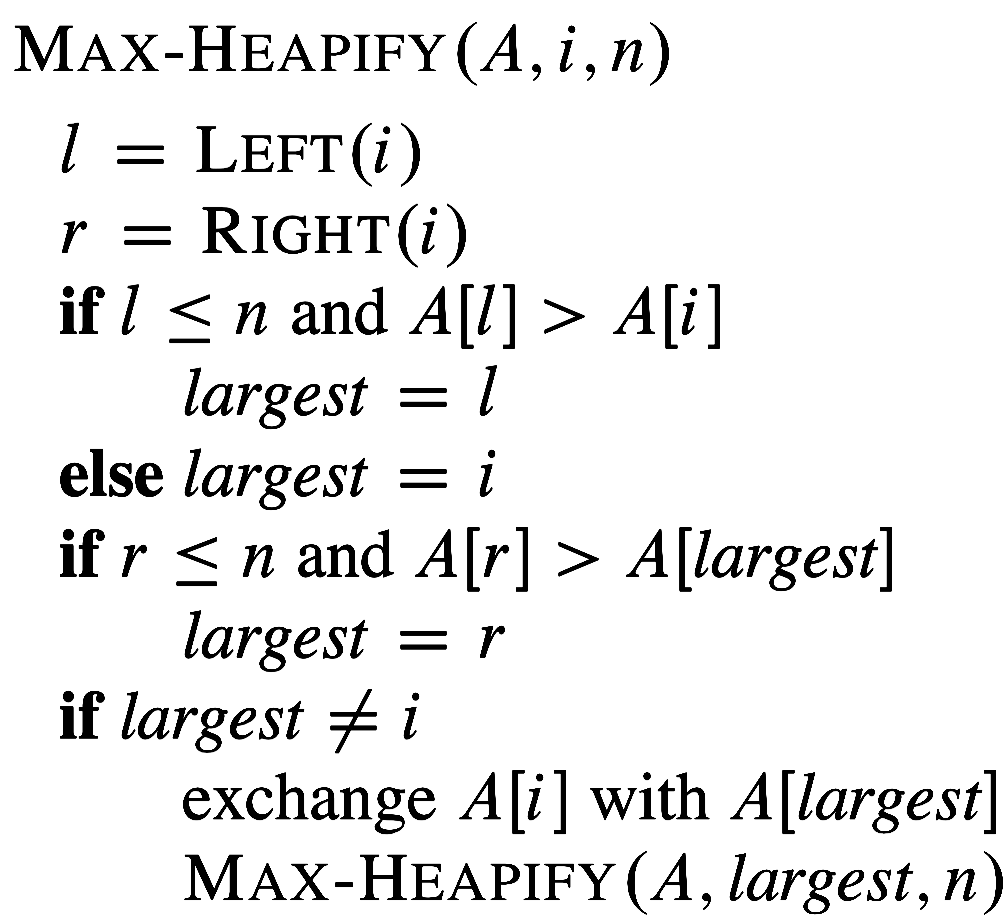
\includegraphics[width=0.7\linewidth]{images/heapify.png}
        \vspace{6pt}
        
        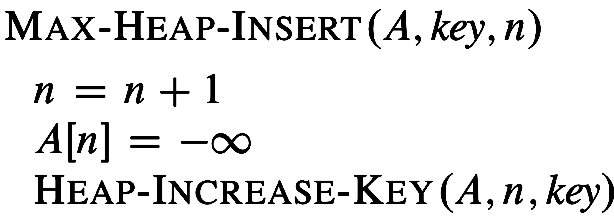
\includegraphics[width=0.7\linewidth]{images/heap-insert.png}
        \vspace{6pt}
        
        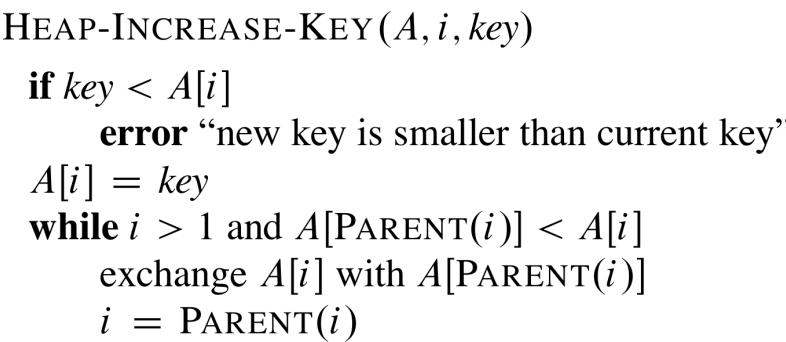
\includegraphics[width=0.7\linewidth]{images/heap-increase-key.png}
        \vspace{6pt}
        
        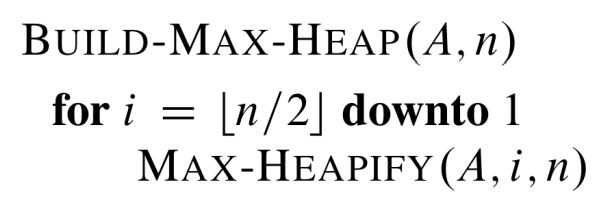
\includegraphics[width=0.7\linewidth]{images/build-max-heap.png}
        \vspace{6pt}
        
        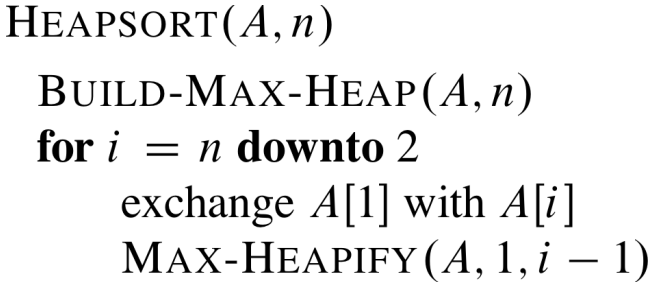
\includegraphics[width=0.7\linewidth]{images/heapsort.png}
    \end{minipage}
}} 
\fbox{
\algoblock{0.6}{\scriptsize Data Structure Operations Summary}{
\tiny
\begin{minipage}[t]{0.49\textwidth}
% Queue Operations
\textbf{\tiny Queue Operations}\\
\begin{tabular}{|p{0.2\textwidth}|p{0.33\textwidth}|p{0.13\textwidth}|p{0.08\textwidth}|}
\hline
\textbf{Operation} & \textbf{Description} & \textbf{Time} & \textbf{Space} \\
\hline
Queue-Empty(Q) & Returns TRUE if queue is empty, FALSE otherwise & $O(1)$ & $O(1)$ \\
\hline
Enqueue(Q, x) & Adds element x to rear of queue Q & $O(1)$ & $O(1)$ \\
\hline
Dequeue(Q) & Removes and returns front element from queue Q & $O(1)$ & $O(1)$ \\
\hline
\end{tabular}\\

% Linked List Operations
\textbf{Linked List Operations}\\
\begin{tabular}{|p{0.2\textwidth}|p{0.33\textwidth}|p{0.13\textwidth}|p{0.08\textwidth}|}
\hline
\textbf{Operation} & \textbf{Description} & \textbf{Time} & \textbf{Space} \\
\hline
List-Search(L, k) & Returns pointer to first node with key k, NULL if not found & $O(n)$ & $O(1)$ \\
\hline
List-Insert(L, x) & Inserts node x at beginning of list L & $O(1)$ & $O(1)$ \\
\hline
List-Delete(L, x) & Removes node x from list L & $O(n)$ find, $O(1)$ del & $O(1)$ \\
\hline
\end{tabular}\\

% Heap Operations
\textbf{Heap Operations}\\
\begin{tabular}{|p{0.2\textwidth}|p{0.3\textwidth}|p{0.16\textwidth}|p{0.08\textwidth}|}
\hline
\textbf{Operation} & \textbf{Description} & \textbf{Time} & \textbf{Space} \\
\hline
Max-Heapify(A, i) & Maintains max-heap property at node i & $O(\log n)$ & $O(1)$ \\
\hline
Build-Max-Heap(A) & Converts array A into max heap & $O(n)$ & $O(1)$ \\
\hline
Heap-Sort(A) & Sorts array A using heap & $O(n \log n)$ & $O(1)$ \\
\hline
Max-Heap-Insert(A, k) & Inserts key k into heap A & $O(\log n)$ & $O(1)$ \\
\hline
Heap-Extract-Max(A) & Returns and removes largest element from heap A & $O(\log n)$ & $O(1)$ \\
\hline
Heap-Increase-Key(A,i,k) & Increases key at index i to new value k & $O(\log n)$ & $O(1)$ \\
\hline
\end{tabular}\\
\end{minipage}
\hspace{-37px}
\begin{minipage}[t]{0.49\textwidth}
\textbf{Stack Operations}\\
\begin{tabular}{|p{0.2\textwidth}|p{0.33\textwidth}|p{0.13\textwidth}|p{0.08\textwidth}|}
\hline
\textbf{Operation} & \textbf{Description} & \textbf{Time} & \textbf{Space} \\
\hline
Stack-Empty(S) & Returns TRUE if stack is empty, FALSE otherwise & $O(1)$ & $O(1)$ \\
\hline
Push(S, x) & Adds element x to top of stack S & $O(1)$ & $O(1)$ \\
\hline
Pop(S) & Removes and returns top element from stack S & $O(1)$ & $O(1)$ \\
\hline
\end{tabular}\\
\textbf{BST Operations}\\
\begin{tabular}{|p{0.2\textwidth}|p{0.33\textwidth}|p{0.13\textwidth}|p{0.08\textwidth}|}
\hline
\textbf{Operation} & \textbf{Description} & \textbf{Time} & \textbf{Space} \\
\hline
BST-Search(T, k) & Finds node with key k in tree T & $O(h)$ & $O(h)$ \\
\hline
BST-Minimum(T) & Returns node with smallest key in T & $O(h)$ & $O(1)$ \\
\hline
BST-Maximum(T) & Returns node with largest key in T & $O(h)$ & $O(1)$ \\
\hline
BST-Successor(x) & Returns node with smallest key greater than x's key & $O(h)$ & $O(1)$ \\
\hline
BST-Insert(T, z) & Inserts node z into BST T & $O(h)$ & $O(1)$ \\
\hline
BST-Delete(T, z) & Removes node z from BST T & $O(h)$ & $O(1)$ \\
\hline
BST-Inorder(T) & Visits all nodes in sorted order & $O(n)$ & $O(h)$ \\
\hline
BST-Preorder(T) & Visits root before its children & $O(n)$ & $O(h)$ \\
\hline
BST-Postorder(T) & Visits children before root & $O(n)$ & $O(h)$ \\
\hline
\end{tabular}\\

% Priority Queue Operations
\textbf{Priority Queue Operations}\\
\begin{tabular}{|p{0.2\textwidth}|p{0.33\textwidth}|p{0.13\textwidth}|p{0.08\textwidth}|}
\hline
\textbf{Operation} & \textbf{Description} & \textbf{Time} & \textbf{Space} \\
\hline
Maximum(S) & Returns element with highest priority & $O(1)$ & $O(1)$ \\
\hline
Extract-Max(S) & Removes and returns element with highest priority & $O(\log n)$ & $O(1)$ \\
\hline
Insert(S, x) & Inserts element x into set S & $O(\log n)$ & $O(1)$ \\
\hline
Increase-Key(S, x, k) & Increases priority of element x to k & $O(\log n)$ & $O(1)$ \\
\hline
\end{tabular}\\
\end{minipage}
}} \\
\fbox{\begin{minipage}[t]{1\textwidth}
   \tiny
    \textbf{Binary Search Trees (BST)}\\[2pt]    
    \begin{minipage}[t]{0.19\textwidth}
        \centering
        \textbf{\scriptsize BST-Search}\\[2pt]
       \tiny
        \begin{minipage}[t]{\textwidth}
           \tiny
            1. Start at root\\
            2. If NULL, return NULL\\
            3. If key = root's key, return root\\
            4. If key < root's key, search left\\
            5. If key > root's key, search right
        \end{minipage}\\[3pt]
        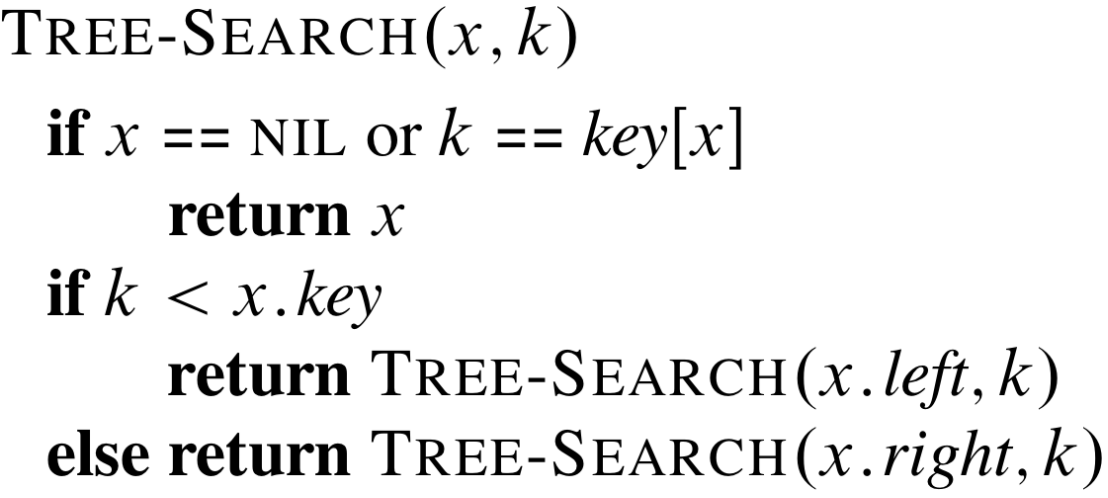
\includegraphics[width=0.85\textwidth]{images/bst-search.png}\\[2pt]
        \textit{Time:} \(O(\log n)\) avg, \(O(h)\) worst\\
        \textit{Space:} \(O(n)\) for tree, \(O(h)\) auxiliary
    \end{minipage}
    \hfill
    \begin{minipage}[t]{0.19\textwidth}
        \centering
        \textbf{\scriptsize BST-Minimum}\\[2pt]
       \tiny
        \begin{minipage}[t]{\textwidth}
           \tiny
            1. Start at root\\
            2. If NULL, return NULL\\
            3. Follow left pointers until no left child\\
            4. Return leftmost node
        \end{minipage}\\[8pt]
        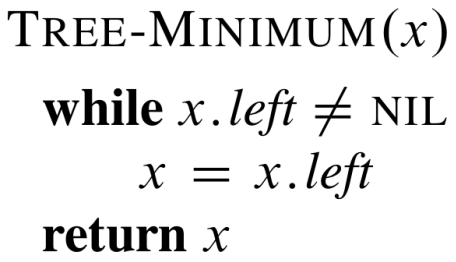
\includegraphics[width=0.5\textwidth]{images/bst-minimum.png}\\[2pt]
        \textit{Time:} \(O(h)\)\\
        \textit{Space:} \(O(n)\) for tree, \(O(1)\) auxiliary
    \end{minipage}
    \hfill
    \begin{minipage}[t]{0.19\textwidth}
        \centering
        \textbf{\scriptsize BST-Maximum}\\[2pt]
       \tiny
        \begin{minipage}[t]{\textwidth}
           \tiny
            1. Start at root\\
            2. If NULL, return NULL\\
            3. Follow right pointers until no right child\\
            4. Return rightmost node
        \end{minipage}\\[8pt]
        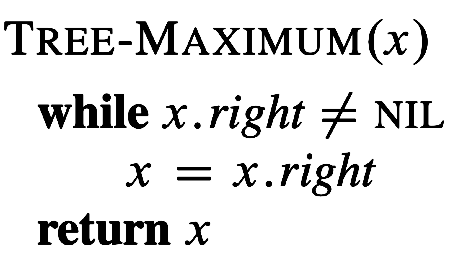
\includegraphics[width=0.5\textwidth]{images/bst-maximum.png}\\[2pt]
        \textit{Time:} \(O(h)\)\\
        \textit{Space:} \(O(n)\) for tree, \(O(1)\) auxiliary
    \end{minipage}
    \hfill
    \begin{minipage}[t]{0.19\textwidth}
        \centering
        \textbf{\scriptsize BST-Successor}\\[2pt]
       \tiny
        \begin{minipage}[t]{\textwidth}
           \tiny
            1. If right subtree exists:\\
            \quad Return minimum in right subtree\\
            2. Otherwise:\\
            \quad Find first ancestor where\\
            \quad node is in left subtree
        \end{minipage}\\[4pt]
        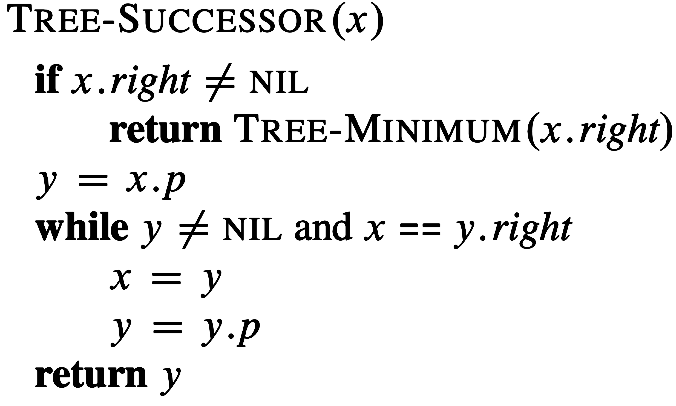
\includegraphics[width=0.8\textwidth]{images/bst-successor.png}\\[2pt]
        \textit{Time:} \(O(h)\)\\
        \textit{Space:} \(O(n)\) for tree, \(O(1)\) auxiliary
    \end{minipage}
    \hfill
    \begin{minipage}[t]{0.19\textwidth}
        \centering
        \textbf{\scriptsize BST-Postorder}\\[2pt]
       \tiny
        \begin{minipage}[t]{\textwidth}
           \tiny
            1. Recursively traverse left\\
            2. Recursively traverse right\\
            3. Visit current node\\
            \textit{(Children first, then root)}
        \end{minipage}\\[4pt]
        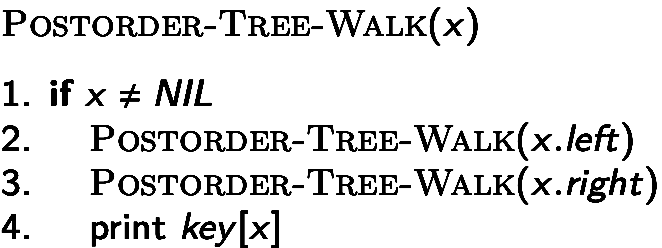
\includegraphics[width=0.8\textwidth]{images/bst-postorder.png}\\[2pt]
        \textit{Time:} \(O(n)\)\\
        \textit{Space:} \(O(n)\) for tree, \(O(h)\) auxiliary
    \end{minipage}
    \hfill
    \begin{minipage}[t]{0.19\textwidth}
        \centering
        \textbf{\scriptsize BST-Inorder}\\[2pt]
       \tiny
        \begin{minipage}[t]{\textwidth}
           \tiny
            1. Recursively traverse left\\
            2. Visit current node\\
            3. Recursively traverse right\\
            \textit{(Visits nodes in sorted order)}
        \end{minipage}\\[4pt]
        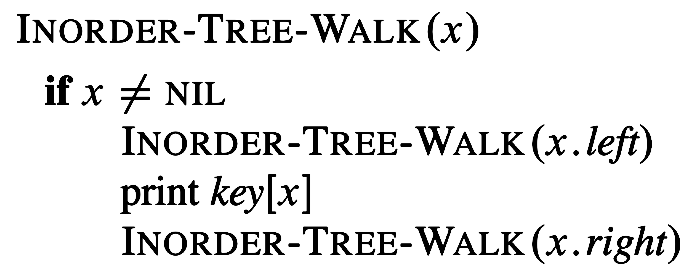
\includegraphics[width=0.8\textwidth]{images/bst-inorder.png}\\[2pt]
        \textit{Time:} \(O(n)\)\\
        \textit{Space:} \(O(n)\) for tree, \(O(h)\) auxiliary
    \end{minipage}
    \hfill
    \begin{minipage}[t]{0.19\textwidth}
        \centering
        \textbf{\scriptsize BST-Preorder}\\[2pt]
       \tiny
        \begin{minipage}[t]{\textwidth}
           \tiny
            1. Visit current node\\
            2. Recursively traverse left\\
            3. Recursively traverse right\\
            \textit{(Root first, then children)}
        \end{minipage}\\[4pt]
        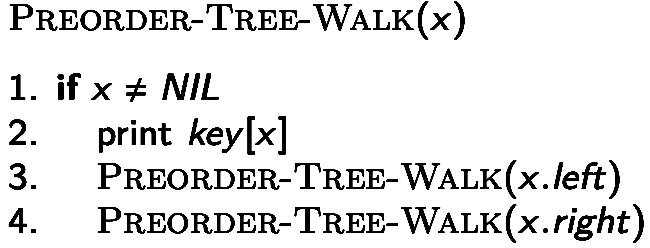
\includegraphics[width=0.8\textwidth]{images/bst-preorder.png}\\
        \textit{Time:} \(O(n)\)\\
        \textit{Space:} \(O(n)\) for tree, \(O(h)\) auxiliary
        \begin{minipage}[t]{1.6\textwidth}
        \hrule
        \end{minipage}
        \vspace{2pt}
        \textbf{Properties:}\\
        \begin{minipage}[t]{1.6\textwidth}
            \begin{itemize}
            \item[-] Left subtree: all keys < node's key
            \item[-] Right subtree: all keys > node's key
            \item[-] Left and right subtrees are also BSTs
            \item[-] A \textbf{Node} has: \textbf{key} (value), \textbf{left} \& \textbf{right} (child pointers), \textbf{parent} (optional)
            \item[-] Tree height \textbf{h}: length of longest path from root to leaf
            \end{itemize}
        \end{minipage}
    \end{minipage}
    \hfill
    \begin{minipage}[t]{0.19\textwidth}
        \centering
        \textbf{\scriptsize BST-Insert}\\[2pt]
       \tiny
        \begin{minipage}[t]{\textwidth}
           \tiny
            1. Create new node z with key\\
            2. Start at root, track parent y = NIL\\
            3. Move down tree (left if key < node key, right otherwise)\\
            4. Once NULL found, link z as child of y\\
            5. If y is NIL, z becomes root\\
            6. Otherwise, insert z as left or right child based on key comparison
        \end{minipage}\\[4pt]
        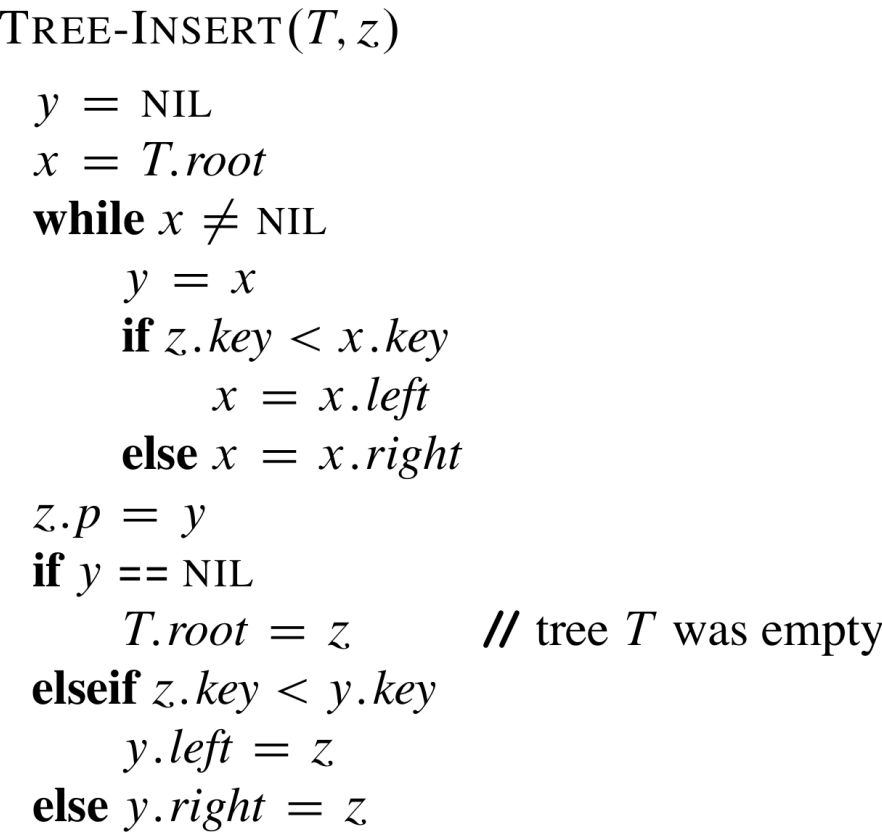
\includegraphics[width=0.8\textwidth]{images/bst-insert.png}\\[2pt]
        \textit{Time:} \(O(h)\)\\
        \textit{Space:} \(O(n)\) for tree, \(O(1)\) auxiliary
    \end{minipage}
    \hfill
    \begin{minipage}[t]{0.19\textwidth}
        \centering
        \textbf{\scriptsize BST-Transplant}\\[2pt]
       \tiny
        \begin{minipage}[t]{\textwidth}
           \tiny
            Replace subtree at u with v:\\
            1. If u is root, set v as root\\
            2. If u is left child, make v left child of u's parent\\
            3. Else make v right child of u's parent\\
            4. Set v's parent to u's parent
        \end{minipage}\\[4pt]
        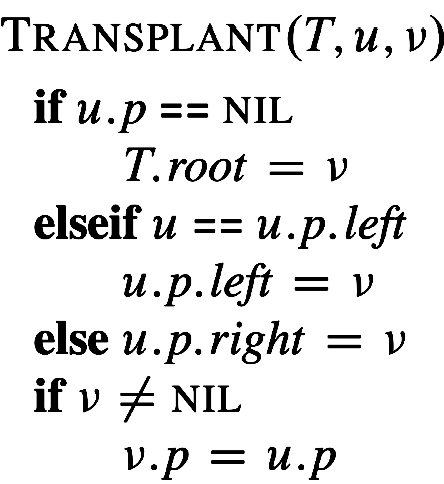
\includegraphics[width=0.4\textwidth]{images/bst-transplant.png}\\[2pt]
        \textit{Time:} \(O(1)\)\\
        \textit{Space:} \(O(n)\) for tree, \(O(1)\) auxiliary
    \end{minipage}
    \hfill
    \begin{minipage}[t]{0.19\textwidth}
        \centering
        \textbf{\scriptsize BST-Delete}\\[2pt]
       \tiny
        \begin{minipage}[t]{\textwidth}
           \tiny
            1. If z has no left: transplant right\\
            2. If z has no right: transplant left\\
            3. With both children:\\
            \quad a. Find successor y\\
            \quad b. Handle y's children\\
            \quad c. Replace z with y
        \end{minipage}\\[4pt]
        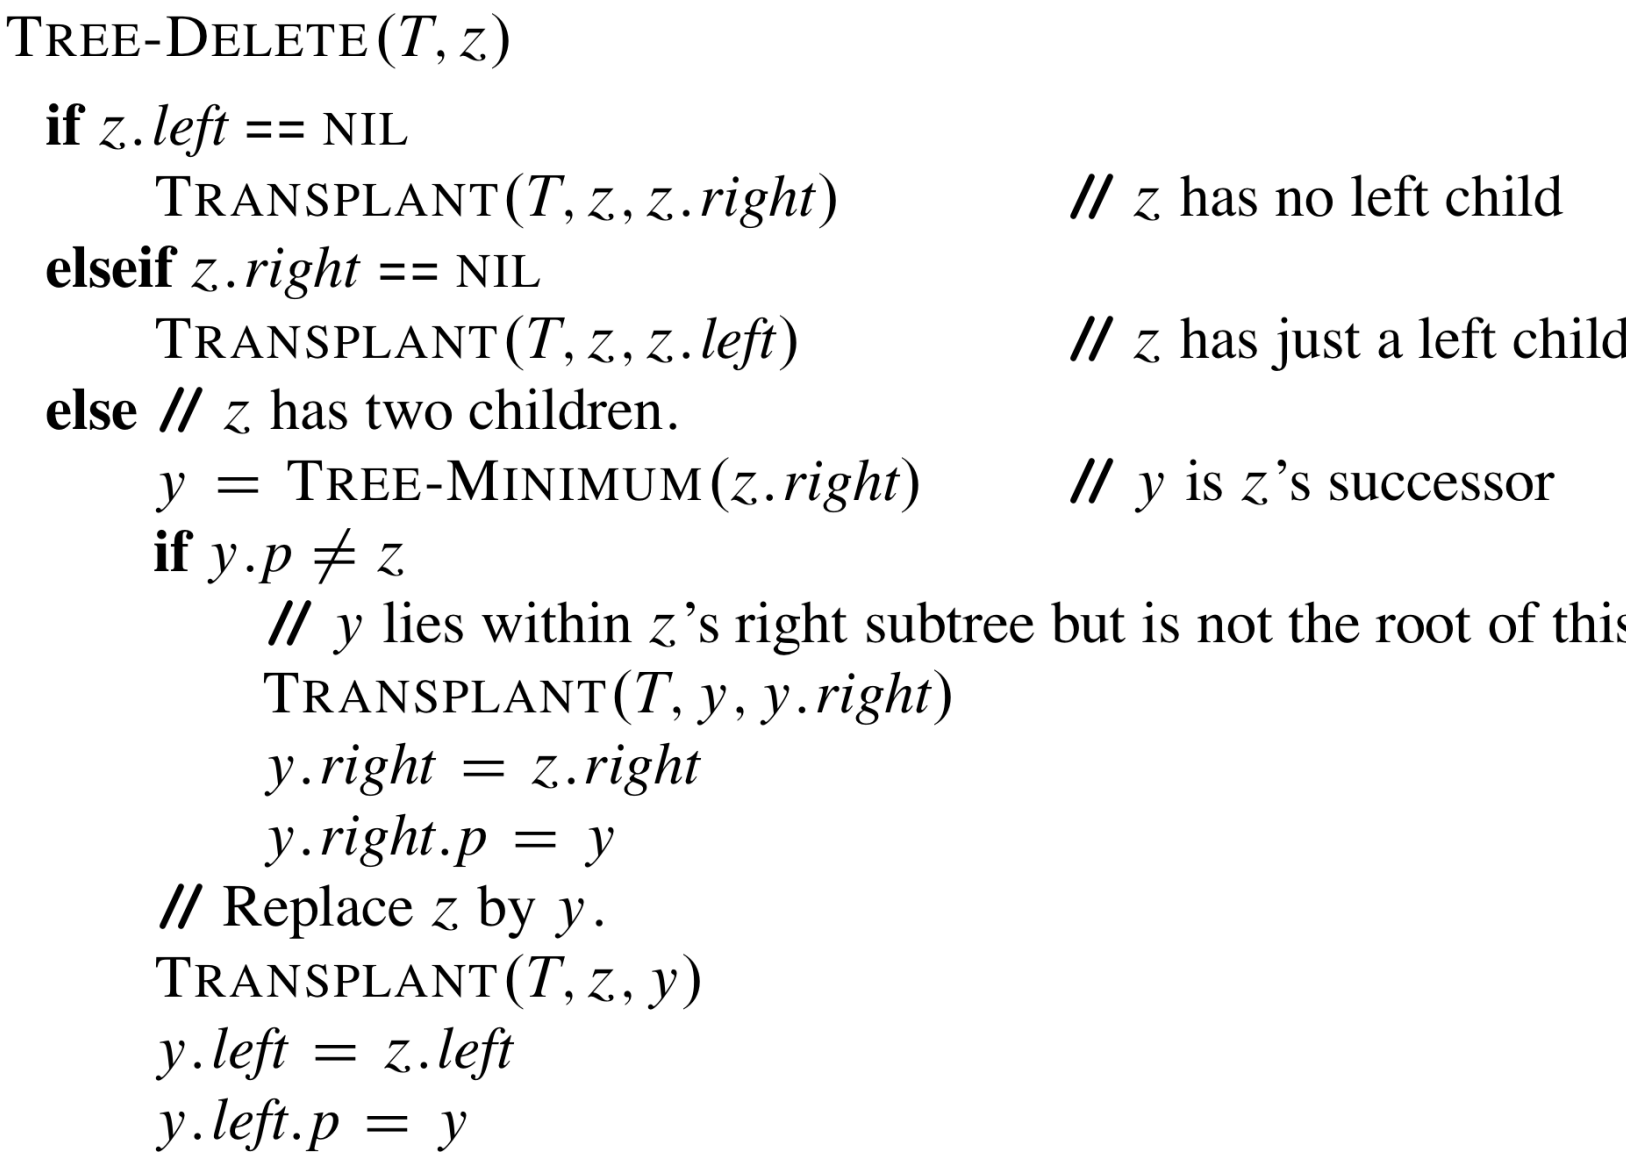
\includegraphics[width=1\textwidth]{images/bst-delete.png}\\[2pt]
        \textit{Time:} \(O(h)\)\\
        \textit{Space:} \(O(n)\) for tree, \(O(1)\) auxiliary
    \end{minipage}
    
    \vspace{2pt}
\end{minipage}} 
\hfill
\fbox{
\algoblock{1}{\scriptsize Dynamic Programming}{
\scriptsize
\begin{minipage}[t]{\textwidth}
\textbf{Problem:} Optimal solutions to overlapping subproblems

\begin{minipage}[t]{0.32\textwidth}
\scriptsize
\textbf{Fibonacci Sequence:}\\
\textbf{Top-Down (Memoization):}\\
1. Create memo array $F[0...n]$ initialized to NIL\\
2. Base cases: $F[0] = 0$, $F[1] = 1$\\
3. Recursive with memo:\\
- Return $F[n]$ if already computed\\
- Otherwise compute $F[n] = F[n-1] + F[n-2]$\\
- Store result in $F[n]$ and return\\[2pt]
\imageblock{1}{images/fib-memoized.png}\\

\textbf{Bottom-Up (Tabulation):}\\
1. Create array $F[0...n]$\\
2. Base cases: $F[0] = 0$, $F[1] = 1$\\
3. For $i = 2$ to $n$:\\
- Compute $F[i] = F[i-1] + F[i-2]$\\
4. Return $F[n]$\\[2pt]
\imageblock{0.45}{images/fib-bottom-up.png}\\
\textbf{Complexity:} Time: $O(n)$, Space: $O(n)$
\end{minipage}
\hfill
\begin{minipage}[t]{0.32\textwidth}
\scriptsize
\textbf{Cut-Rod Problem:}\\
Find optimal way to cut rod to maximize revenue\\
\textbf{Top-Down (Memoization):}\\
1. Create memo array $r[0...n]$ with $r[0] = 0$\\
2. For uncalculated $r[j]$, compute:\\
$r[j] = \max_{1\leq i\leq j}(p[i] + r[j-i])$\\
3. Return $r[n]$\\[2pt]
\imageblock{1}{images/rod-memoized.png}\\

\textbf{Bottom-Up (Tabulation):}\\
1. Create array $r[0...n]$ with $r[0] = 0$\\
2. For $j = 1$ to $n$:\\
- Compute $r[j] = \max_{1\leq i\leq j}(p[i] + r[j-i])$\\
3. Return $r[n]$\\[2pt]
\imageblock{0.5}{images/rod-bottom-up.png}\\
\textbf{Complexity:} Time: $O(n^2)$, Space: $O(n)$
\end{minipage}
\hfill
\begin{minipage}[t]{0.32\textwidth}
\scriptsize
\textbf{Matrix Chain Multiplication:}\\
Find optimal parenthesization to minimize multiplications\\
\textbf{Bottom-Up (Tabulation):}\\
1. Create table $m[1...n, 1...n]$ with $m[i,i] = 0$\\
   - $m[i,j]$ stores minimal cost of multiplying matrices $i$ through $j$\\
2. For $l = 2$ to $n$ (chain length):\\
3. For $i = 1$ to $n-l+1$:\\
- Set $j = i+l-1$\\
- Compute $m[i,j] = \min_{i\leq k<j} \{m[i,k] + m[k+1,j] + p_{i-1}p_kp_j\}$\\
- Store $k$ in $s[i,j]$ that achieved minimum cost\\
4. Return $m[1,n]$\\[2pt]
\imageblock{0.6}{images/matrix-bottom-up.png}\\
\textbf{Complexity:}\\
- Time: $O(n^3)$\\
- Space: $O(n^2)$ for $m$ and $s$ tables\\
- Table $s[i,j]$ stores index of last matrix in first parenthesized group
\end{minipage}
\end{minipage}
}} 
\fbox{
\algoblock{0.45}{\scriptsize Longest Common Subsequence}{
\scriptsize
\begin{minipage}[t]{\textwidth}
\textbf{Problem:} Find the longest subsequence common to two sequences

\begin{minipage}[t]{0.48\textwidth}
\scriptsize
\textbf{LCS-Length:}\\
- Build tables for length $c[0...m, 0...n]$ and direction $b[1...m, 1...n]$\\
- Initialize first row and column to zeros\\
- For each cell $(i,j)$ in the table:\\
\quad If characters match, take diagonal value + 1\\
\quad Otherwise, take maximum from above or left\\
- Table $c[m,n]$ contains the LCS length\\
- Table $b$ records decisions for reconstruction\\[2pt]
\imageblock{0.7}{images/lcs-length.png}
\end{minipage}
\hfill
\begin{minipage}[t]{0.48\textwidth}
\scriptsize
\textbf{Print-LCS:}\\
- Recursively trace back through direction table $b$\\
- Follow diagonal arrows and print characters\\
- Skip cells with up or left arrows\\
- Stops when reaching first row or column\\[2pt]
\imageblock{0.7}{images/print-lcs.png}\\
\scriptsize
\textbf{Example Recording of Solution:}\\
\imageblock{0.7}{images/lcs-table.png}\\

\textbf{Complexity:}\\
- Time: $O(mn)$ for two sequences of lengths $m$ and $n$\\
- Space: $O(mn)$ (includes input sequences and tables)\\
- Space can be optimized to $O(m+n)$ if only length is needed\\
- Print-LCS takes $O(m+n)$ time to reconstruct the solution
\end{minipage}
\end{minipage}
}} 
\fbox{
\algoblock{0.25}{\scriptsize Optimal Binary Search Tree}{
\scriptsize
\begin{minipage}[t]{\textwidth}
\textbf{Problem:} Construct a BST with minimum expected search cost given access probabilities \\
\scriptsize

\textbf{Optimal-BST Algorithm:}
\begin{itemize}[leftmargin=1.2em]
  \item Input: Keys $K_1,\dots,K_n$, probabilities $p_1,\dots,p_n$ for successful searches
  \item Optional: Probabilities $q_0,\dots,q_n$ for unsuccessful searches
  \item Create tables $e[1 \dots n+1,\, 0 \dots n]$ for expected costs
  \item Create $w[i,j]$ for sum of probabilities from $i$ to $j$
  \item Create $root[i,j]$ to record optimal roots
  \item Fill tables bottom‐up by increasing subproblem size
  \item For each subproblem, try all possible roots and pick the minimum cost
  \item Formula: $e[i,j] \;=\; \min_{\,i \le r \le j}\!\bigl\{\,e[i,r-1] \;+\; e[r+1,j] \;+\; w[i,j]\bigr\}$
  \item The root of the overall optimal tree is in $root[1,n]$
\end{itemize}

\imageblock{0.9}{images/optimal-bst.png}
\textbf{Complexity:}
\begin{itemize}[leftmargin=1.2em]
  \item Time: $O(n^3)$ 
  \item Space: $O(n^2)$ for tables $e$, $w$, and $root$
  \item The algorithm computes optimal costs for all possible subtrees
\end{itemize}
\end{minipage}
}} 
\fbox{\begin{minipage}[t]{0.45\textwidth}
    \scriptsize
    \textbf{\scriptsize Linked List}\\
        \scriptsize
        Linear data structure where each node contains: \\
        1. \textbf{key/data}: The value stored in the node \\
        2. \textbf{next}: A pointer to the next node in the sequence \\
        3. \textbf{prev}: A pointer to the previous node (in doubly linked lists) \\
    \textbf{\scriptsize List-Search (find a node with a given key)}\\
    \begin{minipage}[htp]{0.65\textwidth}
        \scriptsize
        1. Start from the head of the linked list.\\
        2. Traverse the list by following the next pointers.\\
        3. Compare each node's key with the target key.\\
        4. Return the node if the key is found.\\
        5. Return NULL if the end of the list is reached without finding the key.
    \end{minipage}
    \begin{minipage}[htp]{0.3\textwidth}
        \begin{center}
            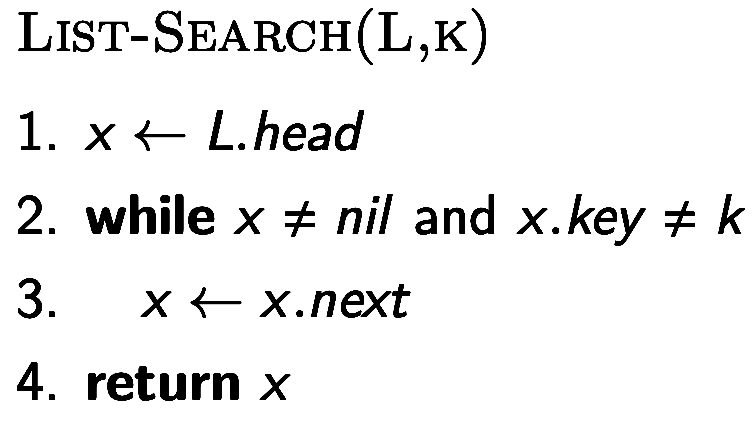
\includegraphics[width=1.1\textwidth]{images/list-search.png}
        \end{center}
    \end{minipage}\\
    \textit{Time Complexity:} \(O(n)\) where n is list length \quad \textit{Space Complexity:} \(O(1)\)\\
    \textbf{\scriptsize List-Insert (insert a new node at the beginning)}\\
    \begin{minipage}[htp]{0.65\textwidth}
        \scriptsize
        1. Create a new node with the given key.\\
        2. Set the next pointer of the new node to point to the current head.\\
        3. If implementing a doubly linked list, set the prev pointer of the current head to the new node.\\
        4. Update the head pointer to point to the new node.\\
        5. If the list was empty, update the tail pointer as well.
    \end{minipage}
    \begin{minipage}[htp]{0.3\textwidth}
        \begin{center}
            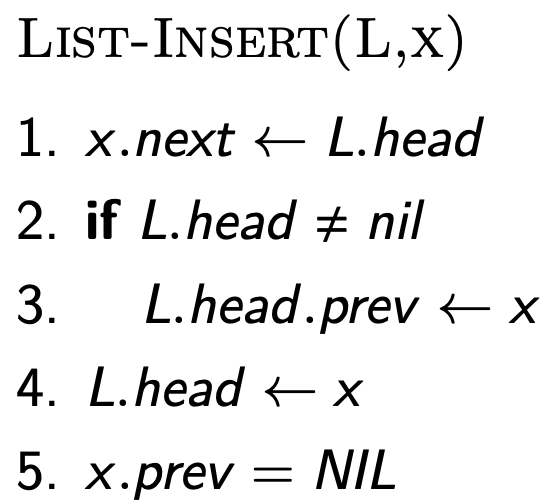
\includegraphics[width=0.9\linewidth]{images/list-insert.png}
        \end{center}
    \end{minipage}\\
    \textit{Time Complexity:} \(O(1)\) \quad \textit{Space Complexity:} \(O(1)\)\\
    \textbf{\scriptsize List-Delete \\(remove a node from the list)}\\
    \begin{minipage}[htp]{0.65\textwidth}
        \scriptsize
        1. Find the node to be deleted (may require traversal).\\
        2. If the node is the head, update the head pointer to the next node.\\
        3. Otherwise, update the next pointer of the previous node to skip the node being deleted.\\
        4. For doubly linked lists, also update the prev pointer of the next node.\\
        5. Free the memory allocated for the deleted node.\\
        6. Handle edge cases: empty list, deleting the only node, or deleting the tail.
    \end{minipage}
    \begin{minipage}[htp]{0.3\textwidth}
        \begin{center}
            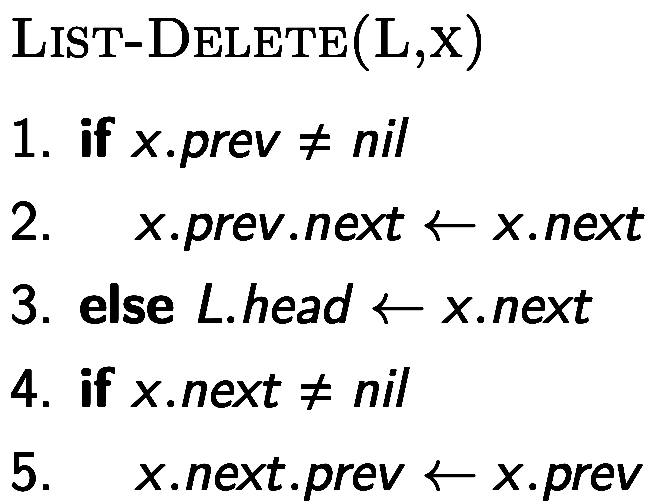
\includegraphics[width=0.9\linewidth]{images/list-delete.png}
        \end{center}
    \end{minipage}\\
    \textit{Time Complexity:} \(O(n)\) for finding the node, \(O(1)\) for deletion \\ \textit{Space Complexity:} \(O(1)\)
\end{minipage}} 
\end{document} 